\documentclass[a4paper,12pt]{report}

\usepackage{alltt, fancyvrb, url}
\usepackage{graphicx}
\usepackage[utf8]{inputenc}
\usepackage{float}
\usepackage{hyperref}

\usepackage[italian]{babel}

\usepackage[italian]{cleveref}

\title{``Donkey Kong''}

\author{Semproli Mattia \\ Foschi Giacomo \\ Di Franco Federico}
\date{10 giugno 2023}


\begin{document}

\maketitle

\tableofcontents

\chapter{Analisi}

\section{Requisiti}

Il progetto a noi commissionato dall'Università di Bologna, si pone l'obiettivo di ricreare un videogioco basato sul classico e celebre Arcade "Donkey Kong (classic)". Rientra nella categoria dei giochi "platformer", ossia videogiochi dove la meccanica di gioco implica l'attraversamento di uno o più livelli, ognuno dei quali composto da piattaforme solitamente situate su più piani.

\subsubsection{Requisiti funzionali}
\begin{itemize}
	\item Il gioco gestirà la partita dell'utente all'interno di un livello composto da piattaforme su più piani, prevederà la presenza di un nemico (donkey kong), barili come ostacoli e di un npc “non playable character” ovvero un personaggio non giocante come traguardo (principessa). 
    \item Un menù iniziale che permetterà l'avvio di una partita e mostrerà una breve legenda dei tasti, incluso anche un tasto quit per chiudere l'applicazione.
    \item Il player durante il gioco potrà muoversi, saltare e salire le scale.
    \item Il gioco implementerà le collisioni tra le entità stesse e anche con i blocchi del livello.
    \item Il gioco prevederà la creazione di power up, positivi e negativi per il player.
    \item Il gioco dovrà gestire la vittoria e la sconfitta.
\end{itemize}

\subsubsection{Requisiti non funzionali}
\begin{itemize}
	\item La grafica di gioco dovrà essere il più coerente possibile all'originale, rimanendo pulita e non confusionaria.
    \item L'interfaccia dovrà essere semplice ed intuitiva.
    \item Si cercherà di offrire una certa fluidità durante il gioco e lo spostamento nel menù, cercando di ottimizzare le prestazioni.
\end{itemize}

\section{Analisi e modello del dominio}

Il gioco è composto da un livello (in un'ottica futura potrebbe prevedere la possibilità di avere più livelli) con una configurazione unica di piattaforme.

Il giocatore dovrà controllare un personaggio e l'obiettivo sarà raggiungere la piattaforma più alta, dove si trova la principessa da salvare, per vincere e concludere la partita. La sfida principale sarà passare da una piattaforma all'altra, utilizzando scale o saltando, evitando contemporaneamente i barili lanciati da Donkey Kong, che si troverà nel livello immediatamente inferiore rispetto a quello della principessa.

Il giocatore avrà un numero limitato di vite, che gli permetteranno di ripartire dalla piattaforma più bassa in caso di collisione con un ostacolo e perdita di una di esse. Quando il giocatore esaurirà tutte le vite, subirà la sconfitta e la partita terminerà. Durante il gioco, saranno disponibili power-up che il giocatore potrà raccogliere per ricevere aiuti extra.

\begin{figure}[H]
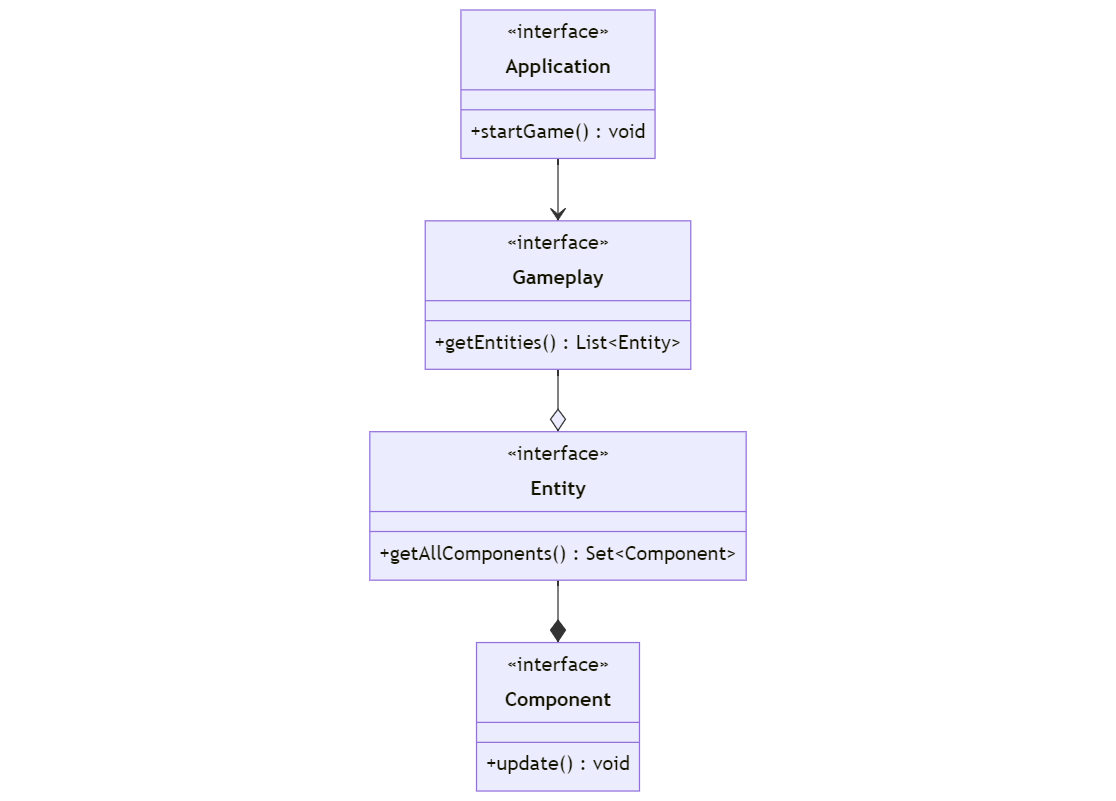
\includegraphics[width=1\textwidth]{img/analisi.png}
\centering{}
\caption{Schema UML dell'analisi del problema, con rappresentate le entità principali ed i rapporti fra loro}
\label{img:analisi}
\end{figure}

\chapter{Design}

\section{Architettura}

Per realizzare il progetto abbiamo adottato il pattern architetturale MVC (Model-View-Controller) cercando di mantenere il più possibile divisi model view e controller. In particolare è composto da: il “model”, che gestisce la logica e i dati del gioco, ed è affidato a tutte le classi contenute all’interno dell’omonima cartella, nella quale è anche presente la parte di ECS che spiegheremo qui di seguito; la “view” che come si può ben intendere gestisce la parte grafica e che in base allo stato di gioco (menu, playing, settings, win, death…) disegnerà la corretta finestra. Anch’essa è collocata all’interno dell’omonima cartella. Infine il “controller”, che ha il compito di interporsi tra model e view per permetterne la comunicazione. A tale scopo è stato creato un controller per ogni stato di gioco. 

Come accennato precedentemente, per la parte di model abbiamo scelto di adottare il pattern ECS (Entity-Component-System). Ogni oggetto di gioco è un’entità caratterizzata dalla presenza o meno di uno o più component, ognuno dei quali descrive uno specifico comportamento. Per esempio un'entità player possiede un MovementComponent che ne gestisce il movimento, ma il quale può essere presente anche in un’altra entità. Questo ci permette di riutilizzare del codice eliminando possibili ripetizioni e rendendo il gioco più flessibile e facilmente estendibile.

\begin{figure}[H]
\centering{}
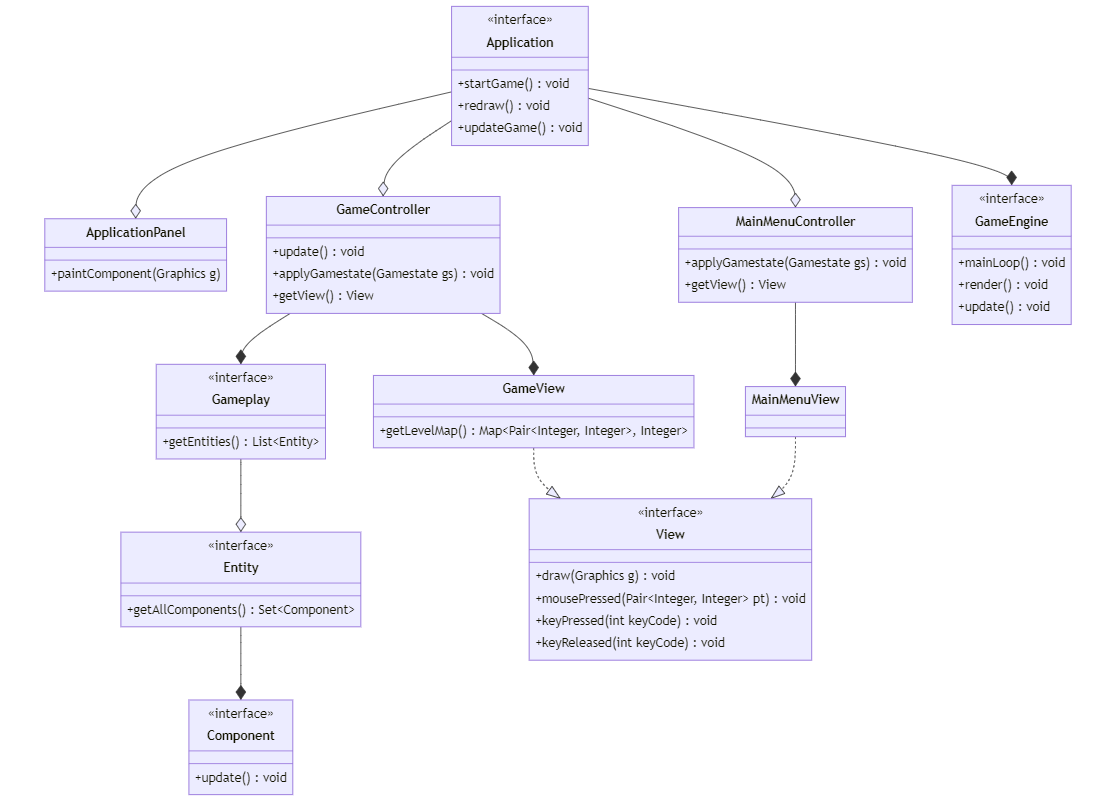
\includegraphics[width=1.25\textwidth]{img/architettura.png}
\caption{Schema UML architetturale di DonkeyKong.}
\label{img:architettura}
\end{figure}

\section{Design dettagliato}
\subsection{Semproli Mattia}

\subsubsection{Gestione del menù}

\begin{figure}[H]
\centering{}
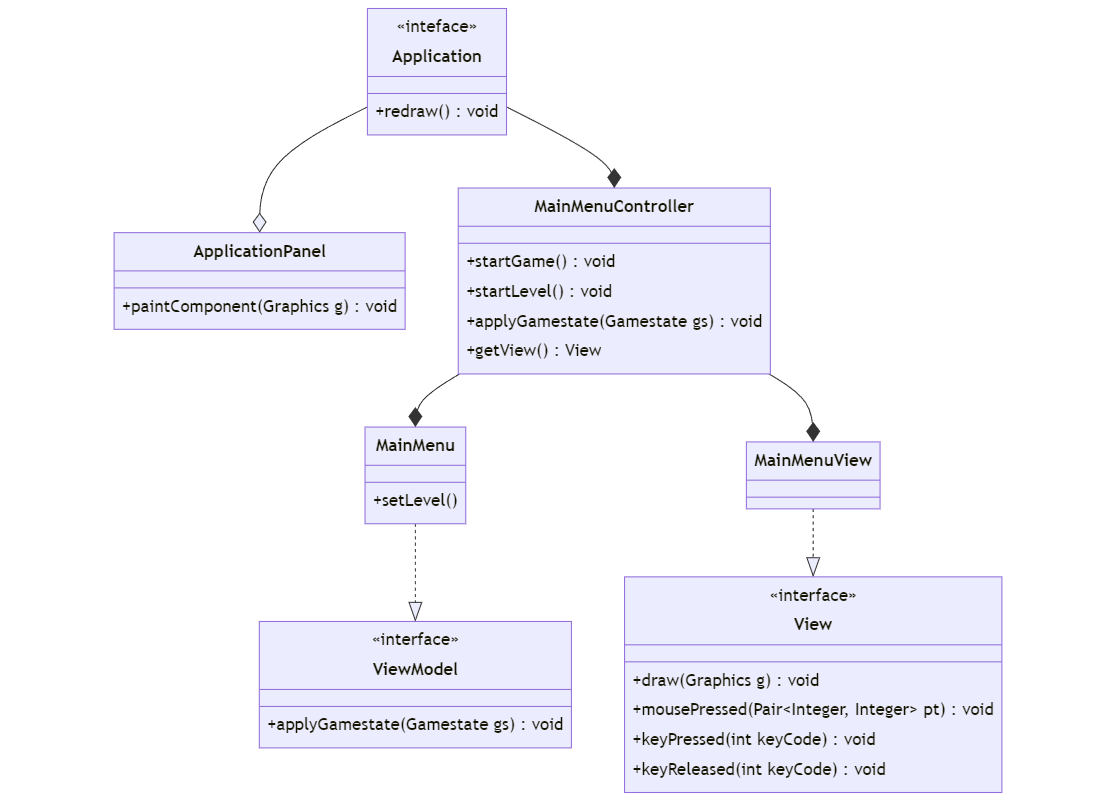
\includegraphics[width=\textwidth]{img/menu.png}
\caption{Rappresentazione UML della gestione MVC per il menu.}
\end{figure}

\paragraph{Problema:}
Il gioco possiede un menù iniziale nel quale è possibile avviare una partita, modificare le impostazioni, scegliere un livello o uscire dal gioco.

\paragraph{Soluzione:}
Voglio iniziare dicendo che le risorse sono già state caricate quando parte l’applicazione, questo vale per tutte le view e stati. Quando viene chiamato draw() all’interno della view saranno disegnati tutti gli elementi grafici dell’attuale stato di gioco, per esempio trovandoci nel menu, il background eccetera. Quando si ottiene un input che sia da mouse o da tastiera, in questo caso per ora solo il primo (il secondo è messo in vista di implementazioni future) in base al bottone che viene premuto sarà notificato al controller uno stato da applicare che sarà passato al model e poi eseguito. In caso il bottone premuto fosse quello che poi ci porta all’inizio di una partita allora sarà settato di default il livello uno, quello considerato iniziale, tramite le chiamate setLevel() e avviata la partita tramite startGame().


\subsubsection{Gestione delle settings}

\begin{figure}[H]
\centering{}

\includegraphics[width=\textwidth]{img/settings.png}
\caption{Rappresentazione UML della gestione MVC per la schermata di settings.}
\end{figure}

\paragraph{Problema:}
Quando ci ritroviamo nella schermata delle impostazioni è possibile tornare al menu, modificare l’audio disattivandolo o attivandolo e cambiare musica di sottofondo.

\paragraph{Soluzione:}
Prettamente simile a quella del Menu, ma con differenza che da questa schermata non ci è permesso avviare una partita; semplicemente quando la view riceverà un punto premuto dal mouse, se sarà sopra un buttone verrà applicato lo stato di riferimento, in caso della pressione dei pulsanti di gestione audio, sarà effettuata l’azione corretta.

\subsubsection{Gestione del menu di scelta dei livelli}

\begin{figure}[H]
\centering{}
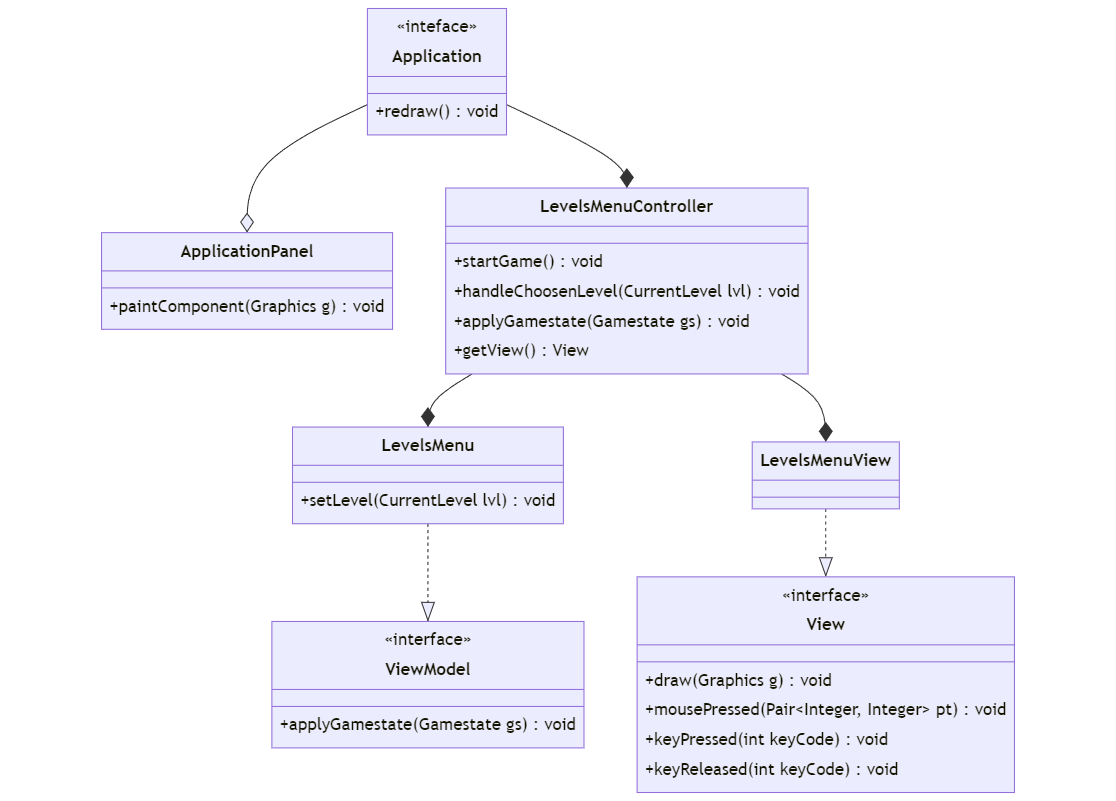
\includegraphics[width=\textwidth]{img/levelsmenu.png}
\caption{Rappresentazione UML della gestione MVC per il menu della scelta del livello.}
\end{figure}

\paragraph{Problema} Nel menu di scelta dei livelli è possibile tornare al menu oppure scegliere un livello.

\paragraph{Soluzione} Come per il Menu, in questa schermata è possibile iniziare una partita, la differenza risiede nel fatto che sono presenti quattro pulsanti diversi (escluso quello per tornare al menu che è uguale in tutte le schermate) che ci permettono di iniziare quattro livelli unici. Quando la view riceve un punto premuto dal mouse, se è stato premuto un pulsante che fa iniziare la partita, viene controllato quale deve essere impostato e inviato al menu. che tramite handleChoosenLevel(CurrentLevel level) lo passa al model che esegue il setLevel(CurrentLevel level). Notiamo in questo caso che a differenza del menu, i metodi sopra citati lavorano con un parametro CurrentLevel (enum per la gestione dei livelli) dato che abbiamo la scelta; ovviamente viene anche chiamato il metodo startGame().

\subsubsection{Gestione della schermata finale e di pausa}

\begin{figure}[H]
\centering{}
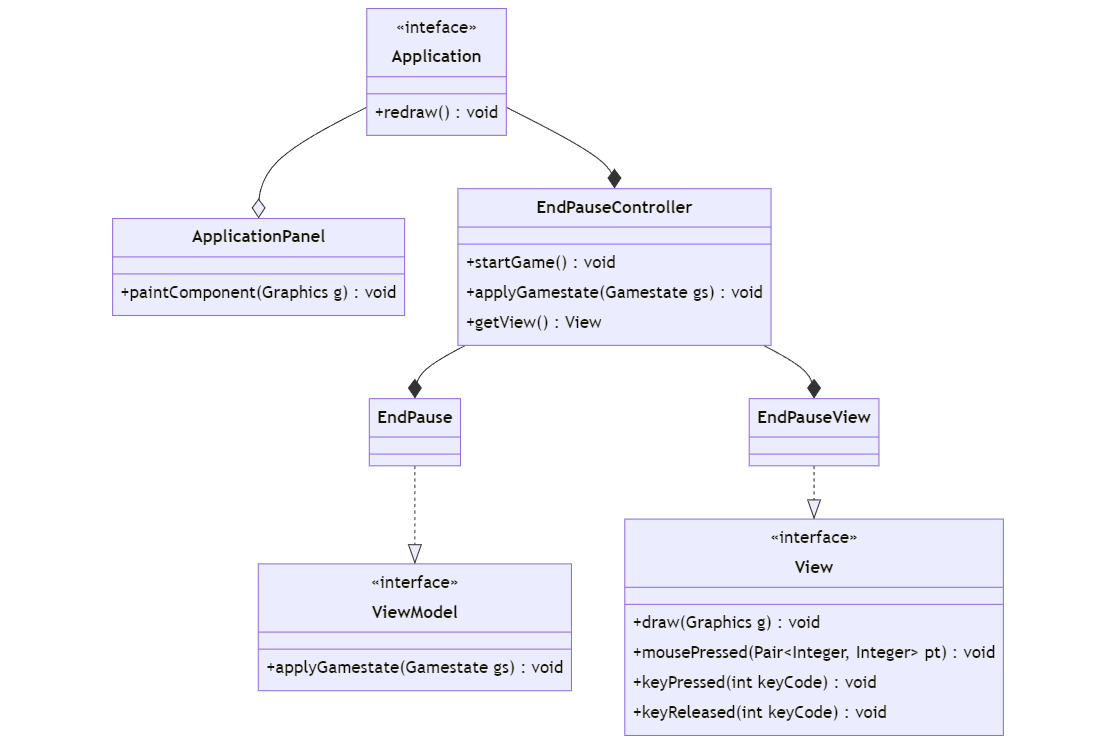
\includegraphics[width=\textwidth]{img/endpause.png}
\caption{Rappresentazione UML della gestione MVC per la schermata finale o di pausa.}
\end{figure}

\paragraph{Problema} Nella schermata di pausa è possibile ritornare al gioco menu, mentre in quella di fine, ovvero vittoria o sconfitta è possibile ricominciare il livello da capo. In entrambe è possibile tornare al menu.

\paragraph{Soluzione} Il pulsante per il Menu funziona come per le altre schermate, in questo caso durante lo sviluppo mi sono reso conto che le schermate erano praticamente tutte identiche, di conseguenza ho deciso di controllare lo stato in cui mi trovo all’interno del draw() in modo da visualizzare solo gli elementi grafici corrispondenti. Il metodo startGame() viene utilizzato quando ci si trova nella schermata di fine, mentre in quella di pausa si procede semplicemente riprendendo la partita in corso. Quando ci si trova nella schermata di pausa sono presenti le stesse impostazioni audio della schermata Settings, semplicmente in questa schermata potremo scegliere tra due musiche di gioco diverse da quelle di menu.

\subsubsection{Gestione della schermata di gioco}

\begin{figure}[H]
\centering{}
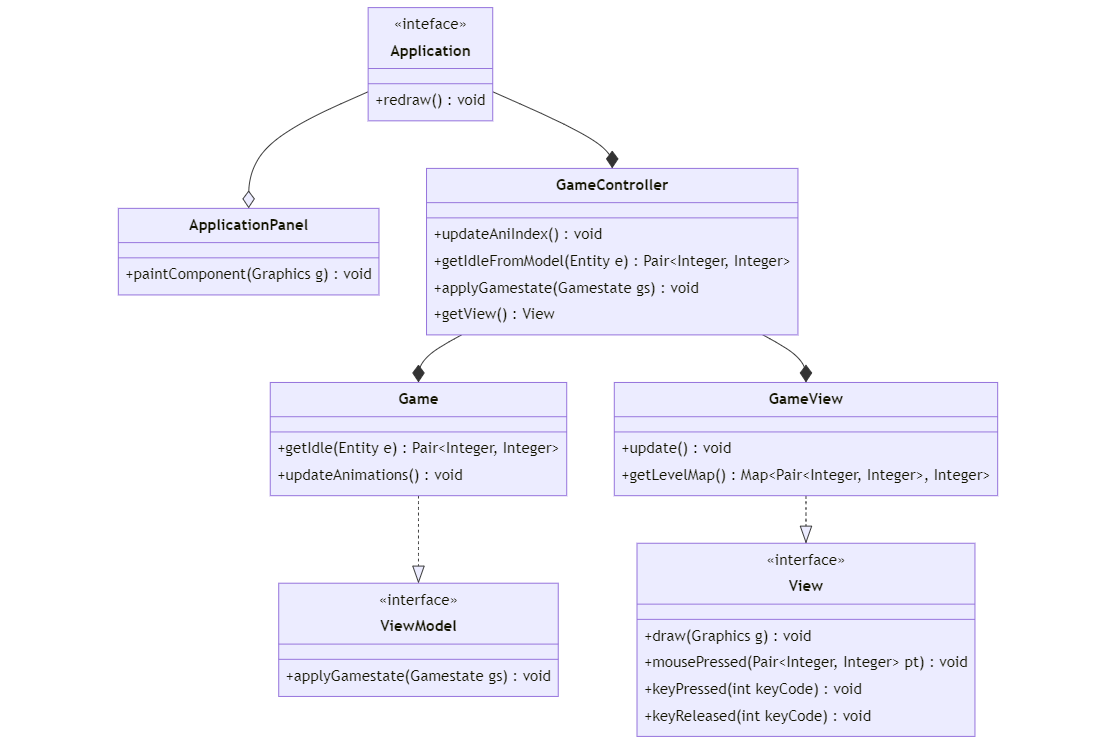
\includegraphics[width=\textwidth]{img/gamecontroller.png}
\caption{Rappresentazione UML della gestione MVC per la schermata di gioco.}
\end{figure}

\paragraph{Problema} Nella schermata di gioco oltre alla possibilità di mettere in pausa il gioco, è necessario a differenza delle altre schermate che possiedono solo sfondi o immagini, caricare e visualizzare graficamente in modo corretto tutte le animazioni e tutti gli sprites. 

\paragraph{Soluzione} Le animazioni sono già caricate come detto in precedenza, poi la GameView tramite getIdle richiede al controller e successivamente al model gli index corretti dell’animazione da mostrare a display. Il metodo update() nella view ci permette di richiedere al controller un aggiornamento da parte del model updateAnimations() di tutti gli indici degli sprite in modo da avere ciclicamente diverse immagini per comporre le animazioni. La view quando viene creata instanzia un oggetto LevelImpl che crea il livello da giocare, è stato inserito nella view dato che utilizzo librerie grafiche per caricare la mappa, mi avvalgo di una immagine pixel per pixel dove in base all’indice RGB, nel nostro caso rosso, ci permette di ottenere la posizione e il tipo di blocco presente. Tramite getLevelMap() si restituiscono solo i valori interi sia delle posizioni che dei blocchi, per poterli poi passare al gameplay al momento della creazione e inizializzare correttamente le entità del livello (per esempio blocco).

\subsubsection{Gestione delle entità}

\begin{figure}[H]
\centering{}
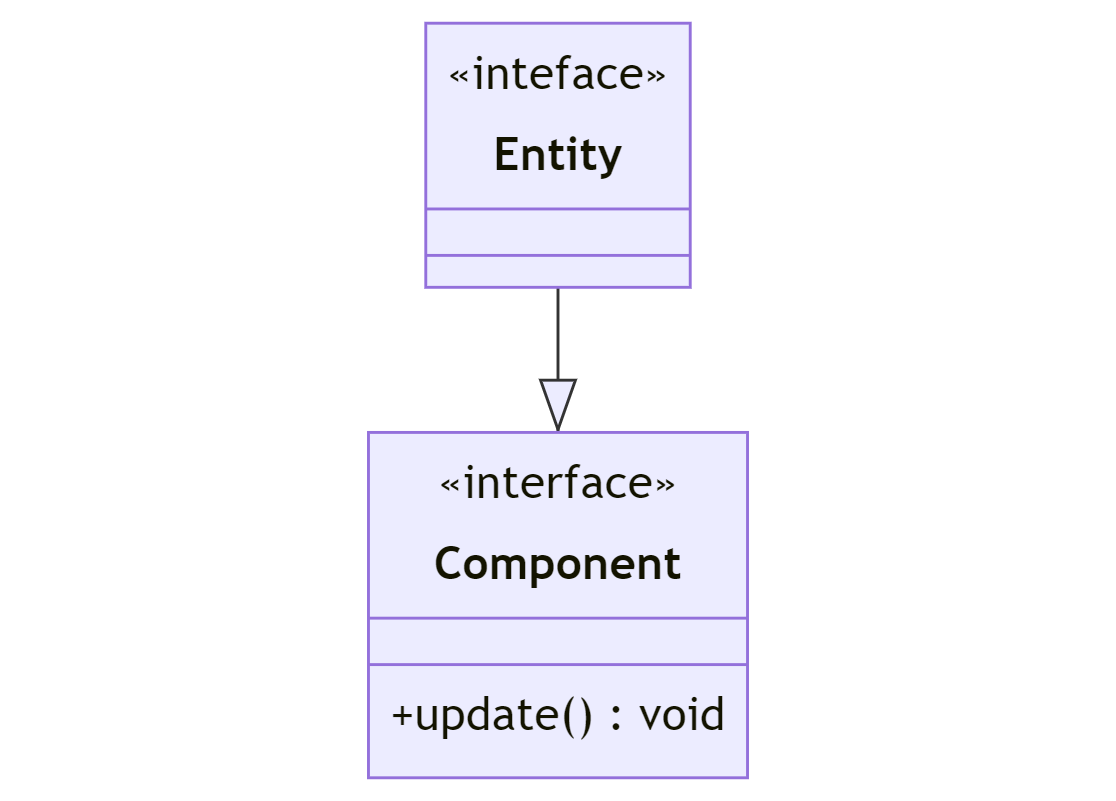
\includegraphics[width=\textwidth]{img/entity.png}
\caption{Rappresentazione UML dell'entità}
\end{figure}

\paragraph{Problema} Le entità sono una parte fondamentale se non il cuore del gioco, di conseguenza ne è opportuna una gestione ottimale, soprattutto considerando il possibile e non raro caso in cui diverse entità possano avere un comportamento uguale o simile.

\paragraph{Soluzione} Per ovviare al problema della ripetizione di codice data da possibili comportamenti simili o uguali, è stato utilizzato il Component Pattern. Ogni entità è un egual guscio vuoto, al quale possiamo aggiungere component specifici o meno durante la creazione. Questo permette un’efficace gestione delle implementazioni delle entità rendendo modifiche, ulteriori implementazioni ed estensioni facilmente apportabili e riutilizzabili.

\subsubsection{Gestione della creazione delle entità}

\begin{figure}[H]
\centering{}
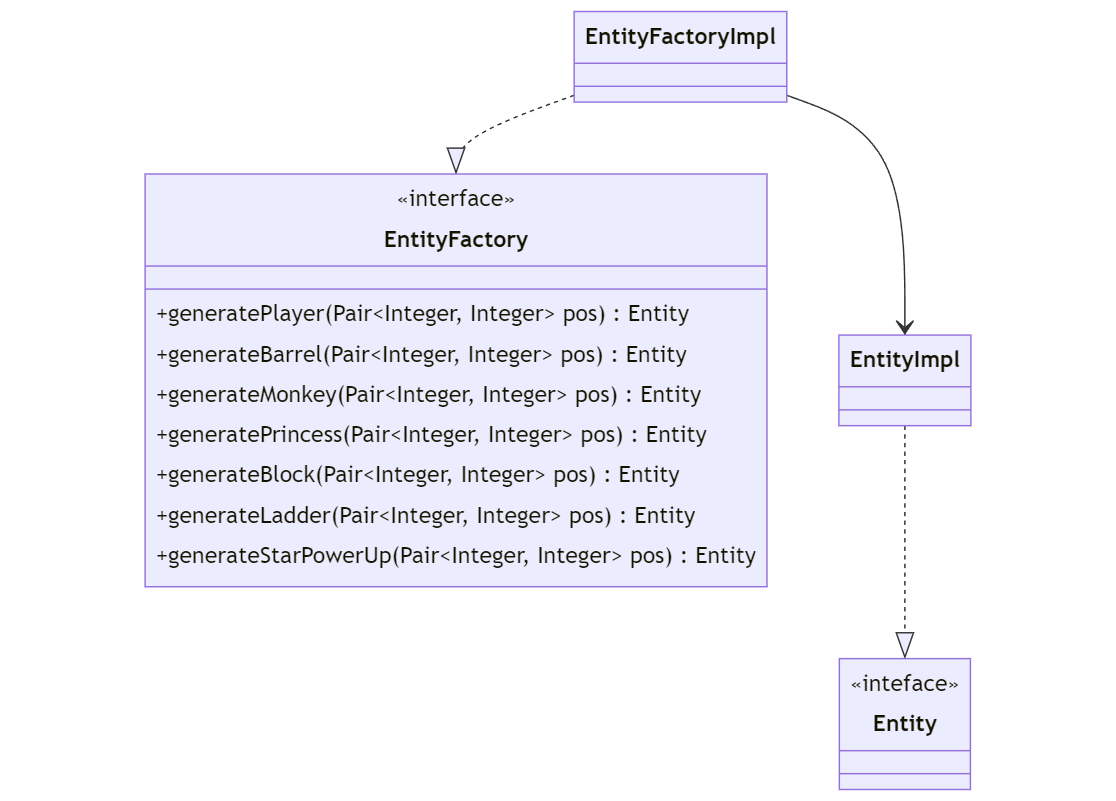
\includegraphics[width=\textwidth]{img/entityfactory.png}
\caption{Rappresentazione UML della creazione delle entità. NB! sono state aggiunte solo alcune di esse.}
\end{figure}

\paragraph{Problema} Sia all’inizio del gioco che durante, è necessario creare diverse entità con diversi component in base ai comportamenti.

\paragraph{Soluzione} Il Factory Pattern ci fornisce un metodo centralizzato per la creazione di nuove istanze di entità, diverse e con component diversi in modo semplice e veloce. Questo ci offre diversi vantaggi, separa la logica di creazione delle entità dal resto dell’applicazione, rendendo il codice più modulare e in caso futuro, di modificare la creazione, i parametri o i component di una o più entità molto più semplicemente. La factory può prendere in ingresso parametri per la creazione di queste entità come per esempio la posizione.

\subsubsection{Gestione delle collisioni}

\begin{figure}[H]
\centering{}
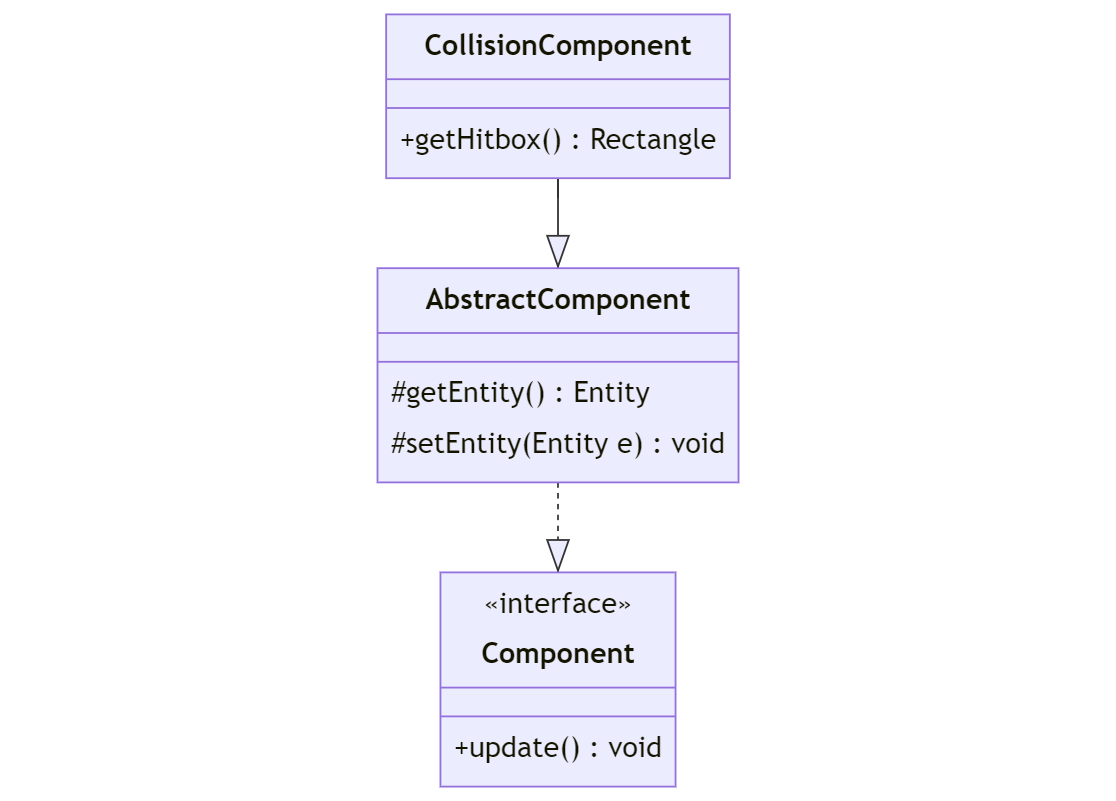
\includegraphics[width=\textwidth]{img/collision.png}
\caption{Rappresentazione UML del collision component.}
\end{figure}

\paragraph{Problema} Il gioco obbligatoriamente deve gestire le varie collisioni tra entità o con i bordi del livello.

\paragraph{Soluzione} Studiando il problema mi sono reso conto che un’ottima soluzione per il controllo delle collisioni fosse predisporre ogni Entità di una hitbox, un oggetto Rectangle che possiede un metodo che mi permette di sapere quando due di essi collidono. Utilizzo il Template Method Pattern, eredito update() da AbstractComponent, che ad ogni richiamo controlla se la relativa entità è in collisione con un’altra gestendone le conseguenze.

\subsection{Foschi Giacomo}

\subsubsection{Gestione del GameEngine}

\begin{figure}[H]
\centering{}
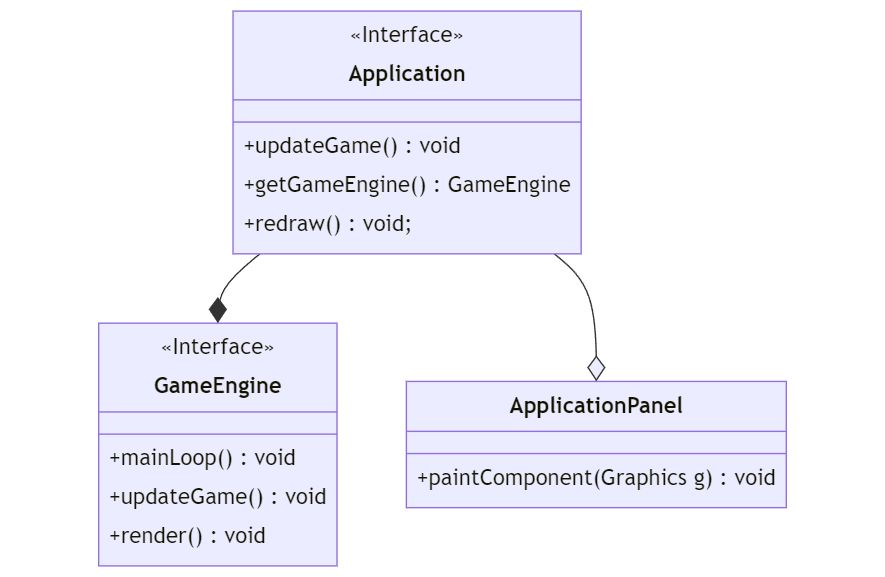
\includegraphics[width=\textwidth]{img/gameloop.jpg}
\caption{Rappresentazione UML del game engine.}
\end{figure}

\paragraph{Problema} Il gioco deve essere in grado di permettere un gameplay fluido senza lag, aggiornando ciclicamente la grafica (view) e la logica di gioco (model) in contemporanea.

\paragraph{Soluzione} Ho deciso di scorporare la gestione del game loop dal controller principale (Application) implementando un’interfaccia GameEngine, al fine di evitare la condivisione di codice sensibile e garantire una maggiore indipendenza, permettendo così di estendere anche in altre classi, in caso di bisogno, il motore del gioco. Il GameEngine viene fatto partire all’avvio dell’applicazione dal controller, richiamando il metodo mainLoop(), nucleo vero e proprio del game che gestisce il ciclo e fa in modo che non si verifichino perdite di frame. Tuttavia, durante lo sviluppo, mi son reso conto che è necessario aggiornare la parte di model e gestione delle varie entità solo nel caso in cui si stia effettivamente giocando; per questa ragione il suddetto metodo prevede che nel caso in cui ci si trovi nel menù iniziale, di pausa, o finale (vittoria o sconfitta), venga aggiornata solo la grafica e non la logica di gioco, risparmiando memoria e processi inutili.

\subsubsection{Gestione di inizio gioco}

\begin{figure}[H]
\centering{}
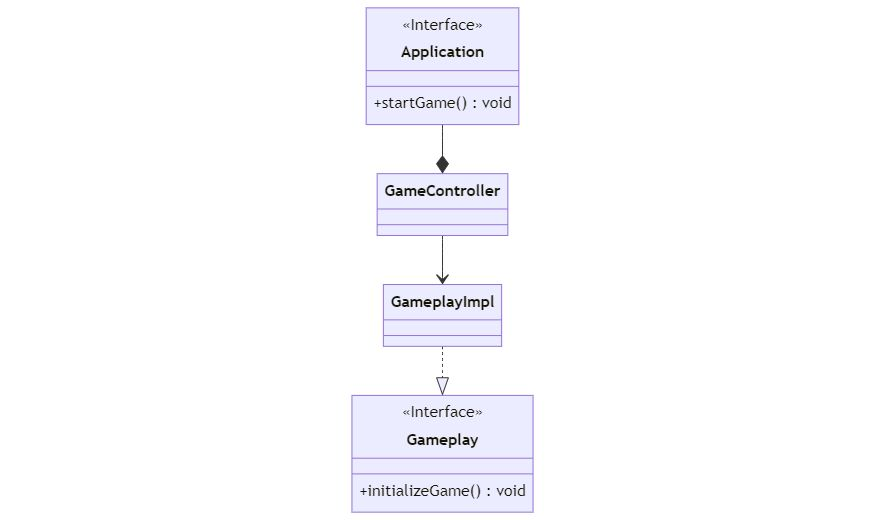
\includegraphics[width=\textwidth]{img/iniziogioco.jpg}
\caption{Rappresentazione UML della logica di inizio gioco.}
\end{figure}

\paragraph{Problema} Avviare una partita in maniera totalmente indipendente ed efficace in qualunque momento e stato dell’applicazione

\paragraph{Soluzione} Per permettere che una nuova partita possa essere sempre iniziata quando viene cliccato il tasto “Play”, ho implementato nel controller principale Application un metodo startGame(). Esso va a creare un nuovo GameController, che si occupa a sua volta di creare un nuovo Gameplay. Attraverso il metodo initializeGame() di quest’ultimo, verranno poi inizializzate tutte le istanze necessarie affinchè si possa giocare una partita.

\subsubsection{Gestione di fine gioco}

\begin{figure}[H]
\centering{}
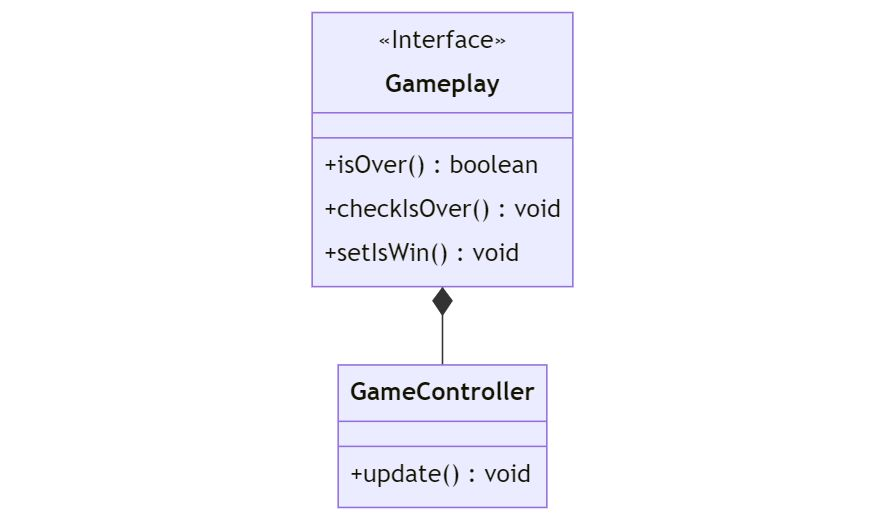
\includegraphics[width=\textwidth]{img/gameplay.jpg}
\caption{Rappresentazione UML della logica di fine gioco.}
\end{figure}

\paragraph{Problema} Controllare che il giocatore abbia perso o vinto una partita.

\paragraph{Soluzione} Per fare in modo che fosse verificata la condizione di vittoria e sconfitta e fosse aggiornato il Gamestate, ho utilizzato un metodo update() all’interno del controller di gioco, che viene eseguito ad ogni ciclo. Questo verifica la condizione di vittoria o sconfitta; se la partita è terminata, aggiorna solamente la grafica senza aggiornare le entità. Per fare ciò, richiama i metodi del gameplay checkIsOver(), isOver(), e setIsWin(). I primi due verificano che esista ancora un player nella lista delle entità di gioco: nel caso non esistesse, cambia il Gamestate in Death e fermano il timer di gioco. Il terzo, è un metodo che viene richiamato all’interno delle Collision quando l’entità del player va a collidere con la principessa, e setta il Gamestate a Win (fermando anch’esso il timer di gioco).

\subsubsection{Gestione dei barili}

\begin{figure}[H]
\centering{}
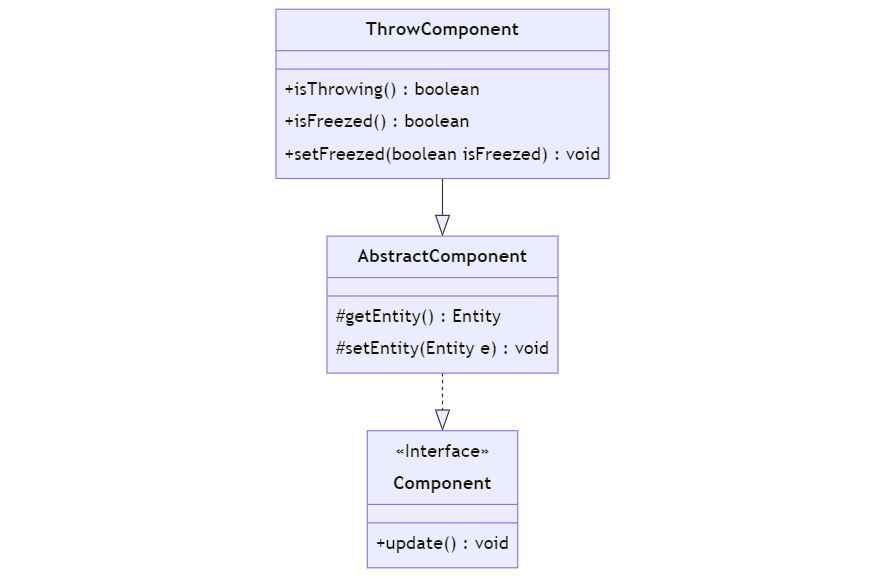
\includegraphics[width=\textwidth]{img/throw.jpg}
\caption{Rappresentazione UML della logica di spawn dei barili.}
\end{figure}

\paragraph{Problema} Gestione dello spawn dei barili durante la partita.

\paragraph{Soluzione} Per gestire la generazione delle entità barili durante la partita da parte del nemico (Donkey Kong), ho implementato un Component da associare esso, sfruttando così il Template Method Pattern, ereditando update() da AbstractComponent. Questo verifica se DK si trova in uno stato di congelamento per via di un powerup, e quindi se non deve generare barili, o se al contrario gli è concesso lanciare gli ostacoli.

\subsection{Di Franco Federico}

\subsubsection{Gestione powerup}

\begin{figure}[H]
\centering{}
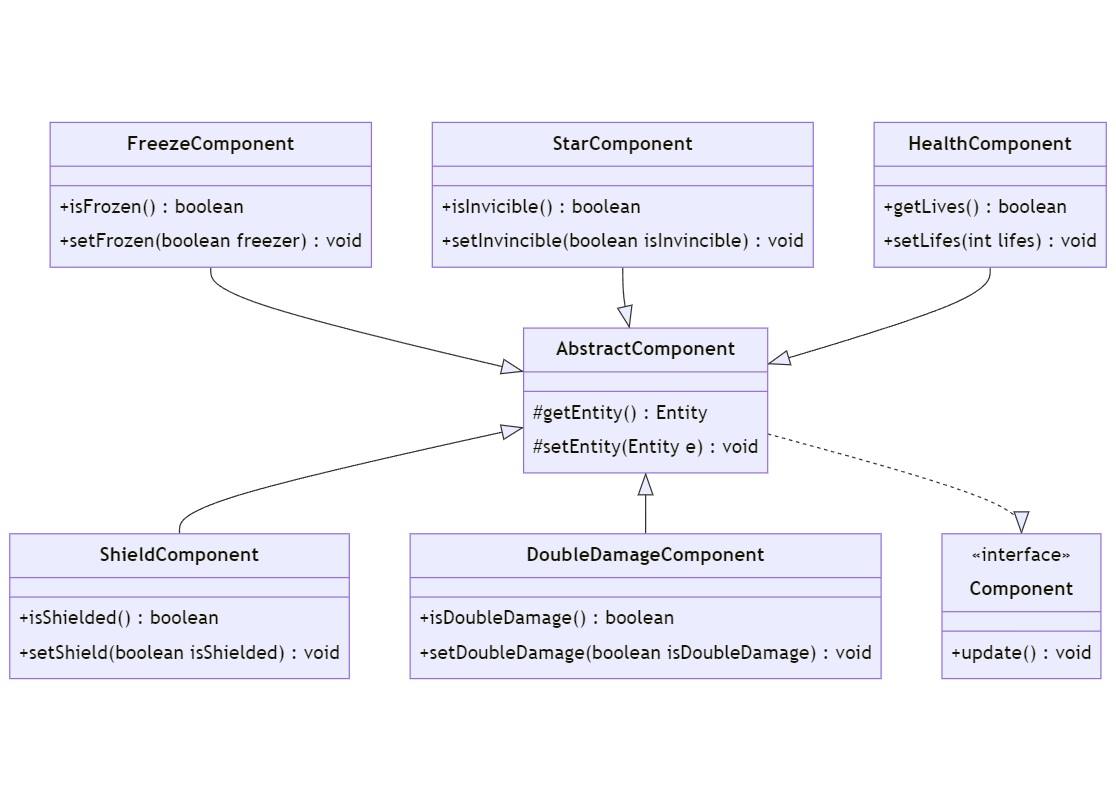
\includegraphics[width=\textwidth]{img/somepowerups.jpg}
\caption{Rappresentazione UML dei power ups.}
\end{figure}

\paragraph{Problema} Il giocatore deve poter usufruire di eventuali powerup sparsi per la mappa i quali forniscono potenziamenti. Anche i barili possono avere powerup, come il danno doppio.

\paragraph{Soluzione} Ho deciso di creare un component per ogni powerup, in modo da ottenere una gestione semplice, efficace e facilmente estendibile, ognuno di essi eredita update() da AbstractComponent sfruttando il Template Method Pattern. Ognuno di essi ha un metodo set e get: tramite il primo impostiamo lo stato del power up, il secondo ci ritorna lo stato stesso. Si nota che tra i power up presenti c'è anche SlowComponent, il quale però non viene mai effettivamente utilizzato, questo perchè è stato inserito in vista futura. In ogni caso per poterlo utilizzare basterebbe semplicemente aggiungerlo ad un entità.

\subsubsection{Gestione listener generici di input da tastiera e mouse}

\begin{figure}[H]
\centering{}
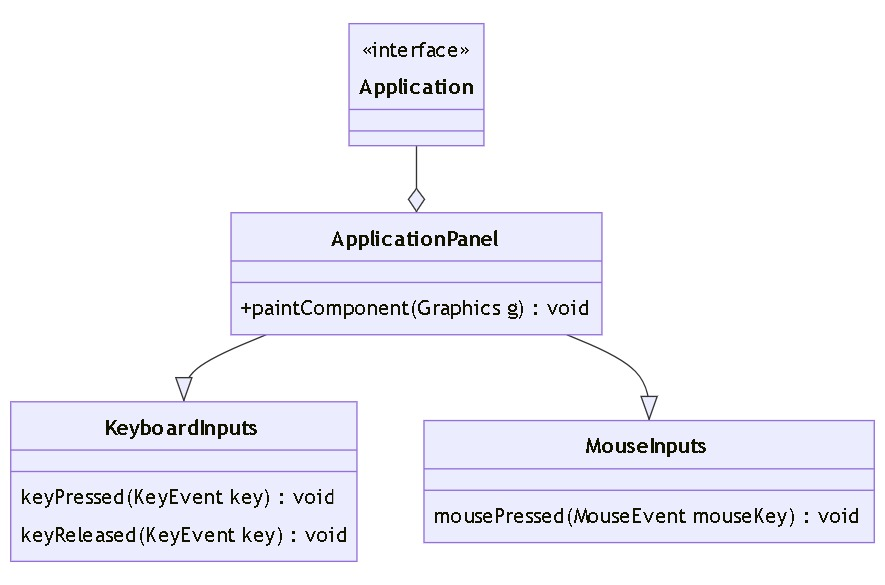
\includegraphics[width=\textwidth]{img/input.jpg}
\caption{Rappresentazione UML del mouse e keyboard input listener.}
\end{figure}

\paragraph{Problema} Notificare le view quando avviene un mouse event o un key event.

\paragraph{Soluzione} Siccome ogni view può ricevere gli stessi eventi, abbiamo deciso di creare due listener generici MouseInputs e KeyboardInputs. Essi vengono aggiunti alla classe ApplicationPanel, quando riceveranno un evento, in base allo stato di gioco, lo invieranno alla corretta view. Se è un input da tastiera, sarà inviato come codice intero, nell’altro caso, sarà inviata una coppia di interi con le coordinate x e y del punto premuto dal mouse. Quando durante il gioco avviene la pressione di un tasto che corrisponde ad un movimento, sarà notificato al GameController che si preoccuperà di passarlo al Gameplay in modo tale da aggiungerlo alla lista di tasti premuti, da processare successivamente nell’input component. Utilizziamo una lista di tasti in modo da evitare ipotetici inconvenienti come la perdita di un tasto dovuto al lag.

\subsubsection{Gestione degli input del player InputsComponent}

\begin{figure}[H]
\centering{}
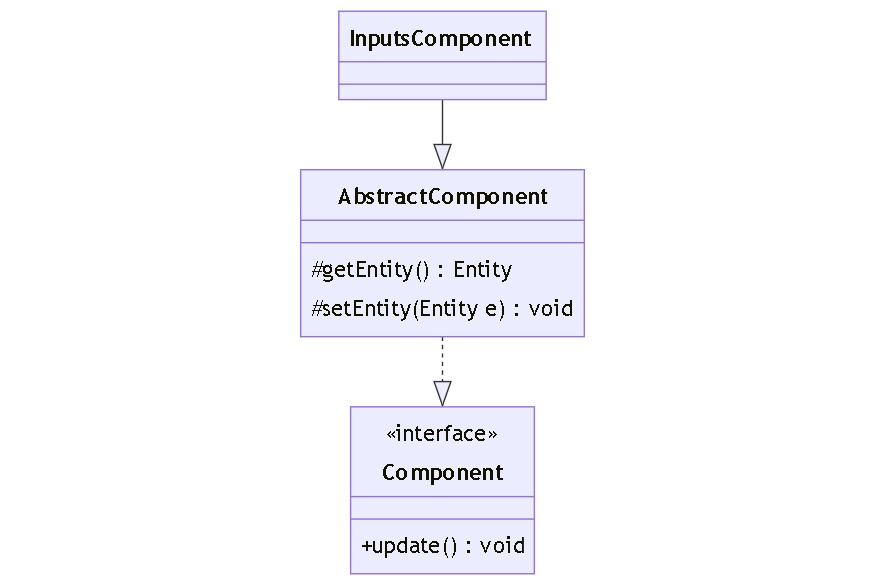
\includegraphics[width=\textwidth]{img/inputscomponent.jpg}
\caption{Rappresentazione UML della logica dell'inputs component.}
\end{figure}

\paragraph{Problema} Durante il gioco è necessario aggiornare gli input da tastiera per poter far muovere il nostro player.

\paragraph{Soluzione} Per gestire gli input, ho deciso di creare un component apposito. L’unico metodo che possiede è l’update() ereditato da AbstractComponent adottando Template Method Pattern, dove ad ogni chiamata tramite la relativa entità ottiene la lista di input da processare, se non è vuota si salva il primo presente, il quale poi viene controllato in modo da poter assegnare l’azione corretta al MovementComponent.

\subsubsection{Gestione movimento entità:}

\begin{figure}[H]
\centering{}
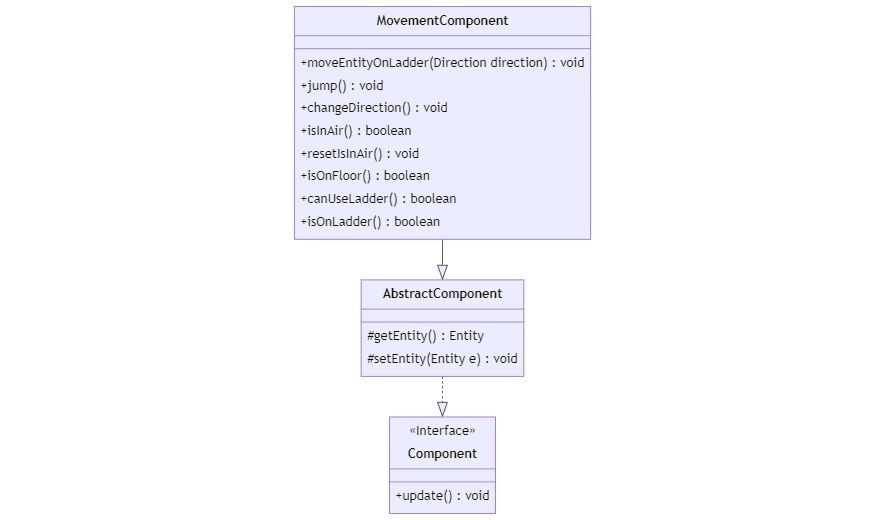
\includegraphics[width=\textwidth]{img/movement.jpg}
\caption{Rappresentazione UML della logica di movimento.}
\end{figure}

\paragraph{Problema} Gestire correttamente i movimenti delle varie entità.

\paragraph{Soluzione} Ho creato un component per il movimento, in modo che in caso di aggiunta di entità che possono muoversi sia sufficiente aggiungerlo durante la loro creazione. Tramite i metodi moveEntityOnLadder(), moveEntity() e jump() è possibile muovere e far eseguire la corretta azione all’entità: durante l'update() ereditato da AbstractComponent (Template Method Pattern) verrà assegnata ad essa una posizione fittizia, che ho deciso di non impostare immediatamente come nuova posizione, al fine di evitare spostamenti illeciti. Sarà successivamente compito del collision component assegnarne la posizione definitiva.


\chapter{Sviluppo}
\section{Testing automatizzato}

Per realizzare i seguenti test è stato utilizzato JUnit 5:
\begin{itemize}
 \item TimerTest, controlla il corretto funzionamento del timer.
 \item InputsComponentTest, controlla il corretto funzionamento degli input da tastiera.
 \item BarrelTest, controlla la corretta creazione di un barile normale e di tipo danno doppio (ossia con DoubleDamageComponent).
 \item CollisionTest, controlla il funzionamento delle collisioni entità-entità e entità-blocchi.
 \item GameplayTest, controlla la corretta inizializzazione di un gameplay e le conseguenti situazioni di vittoria e sconfitta.
 \item MonkeyTest, controlla la corretta creazione di un nemico (Donkey Kong) e delle sue funzionalità.
 \item PlayerTest, controlla la corretta creazione di un player, del suo movimento (incluso il salto) e verifica che si ottengano i giusti component quando richiesti.
 \item PowerupTest, controlla la creazione dei vari powerups e il loro corretto funzionamento.
\end{itemize}

\section{Metodologia di lavoro}
Abbiamo deciso di lavorare a questo progetto utilizzando DVCS come spiegato a lezione, clonando il repository git ognuno in locale per poter lavorare individualmente; in seguito, abbiamo condiviso i cambiamenti effettuati al codice tramite i comandi pull e push.

Prima di iniziare a sviluppare l'applicazione, abbiamo designato le interfacce principali e la suddivisione del lavoro equamente in modo da poter lavorare indipendentemente, cooperando solo per alcune implementazioni (quali ad esempio le collisioni e il movimento), ciascuno su una propria parte di model.

\subsection*{Semproli Mattia}

In autonomia mi sono occupato di:
\begin{itemize}
    \item Grafica di gioco (completa gestione di donkeykong.view.impl e donkeykong.view.api) 
    \begin{itemize}
        \item Per la gestione del corretto sprite di una certa animazione del player ho creato l’enum PlayerIdle (in donkeykong.utilities)
        \item Creazione dell’enum CurrentLevel (in donkeykong.utilities)
    \end{itemize}
    \item Model e Controller relativi alle view (in donkeykong.controller e donkeykong.model.impl)
    \item L’implementazione delle entità (in donkeykong.model.ecs)
    \item Creazione di AbstractComponent (in donkeykong.model.ecs)
    \item Gestione audio e resources (AudioUtilities e ResourceFuncUtilities in donkeykong.utilities)
\end{itemize}

In collaborazione con entrambi:
\begin{itemize}
    \item CollisionComponent (in donkeykong.model.ecs.impl)
    \item Gestito la creazione delle entità all’interno di EntityFactoryImpl (in donkeykong.model.impl)
\end{itemize}

\subsection*{Foschi Giacomo}
In autonomia mi sono occupato di:
\begin{itemize}
    \item GameEngine (package donkeykong.game.core)
    \item Gestione del controller principale Application e inizializzazione del gioco (in donkeykong.controller)
    \item Gestione vittoria e sconfitta nel gameplay (in donkeykong.model)
    \item Gestione nel GameController dell’update durante il gioco (in donkeykong.controller)
    \item Gestione dei barili tramite ThrowComponent (in donkeykong.model.ecs.impl)
    \item Gestione del timer (in donkeykong.common)
\end{itemize}

In collaborazione con Semproli:
\begin{itemize}
    \item Creazione dell’enum Gamestate (in donkeykong.utilities)
\end{itemize}

In collaborazione con entrambi:
\begin{itemize}
    \item Gestione del gameplay generale (in donkeykong.model)
\end{itemize}

\subsection*{Di Franco Federico}
In autonomia mi sono occupato di:
\begin{itemize}
    \item Gestione listener generici di input da tastiera e mouse (in donkeykong.view.inputs)
    \item Gestione dei power up
    \begin{itemize}
        \item StarComponent
        \item ShieldComponent
        \item FreezeComponent
        \item DoubleDamageComponent
        \item HealthComponent (tutti in donkeykong.model.ecs.impl)
    \end{itemize}
    \item Gestione degli input del player InputsComponent (in donkeykong.model.ecs.impl)
    \item Creazione dell’enum Direction (in donkeykong.utilities)
\end{itemize}

In collaborazione con entrambi:
\begin{itemize}
    \item Gestione del movimento MovementComponent (in donkeykong.model.ecs.impl)
\end{itemize}

\subsection*{In gruppo abbiamo fatto:}
\begin{itemize}
    \item Gestito i due file di constanti ModelConstants e ViewConstants (in donkeykong.utilities)
    \item Creazione dell’enum Type contenente i tipi di entità (in donkeykong.utilities)
\end{itemize}

\section{Note di sviluppo}
\subsection*{Semproli Mattia}

\subsubsection{Utilizzo di \texttt{Optional}}
Permalink:
\begin{itemize}
    \item \url{https://github.com/MattiaSemproli/OOP22-DonkeyKong/blob/main/src/main/java/it/unibo/donkeykong/model/ecs/impl/CollisionComponent.java#L29}
\end{itemize}

\subsubsection{Utilizzo di \texttt{Stream} e lambda expressions}
Permalink:
\begin{itemize}
    \item \url{https://github.com/MattiaSemproli/OOP22-DonkeyKong/blob/main/src/main/java/it/unibo/donkeykong/model/ecs/impl/CollisionComponent.java#L87-L108}
    \item \url{https://github.com/MattiaSemproli/OOP22-DonkeyKong/blob/main/src/main/java/it/unibo/donkeykong/view/impl/GameView.java#L87-L93}
\end{itemize}

\subsection*{Foschi Giacomo}
\subsubsection{Utilizzo di \texttt{Optional}}
Permalink:
\begin{itemize}
    \item \url{https://github.com/MattiaSemproli/OOP22-DonkeyKong/blob/main/src/main/java/it/unibo/donkeykong/model/ecs/impl/CollisionComponent.java#L52}
\end{itemize}

\subsubsection{Utilizzo di \texttt{Stream} e lambda expressions}
Permalink:
\begin{itemize}
    \item \url{https://github.com/MattiaSemproli/OOP22-DonkeyKong/blob/main/src/main/java/it/unibo/donkeykong/controller/impl/GameController.java#L49}
    \item \url{https://github.com/MattiaSemproli/OOP22-DonkeyKong/blob/main/src/main/java/it/unibo/donkeykong/model/impl/GameplayImpl.java#L245-L249}
\end{itemize}

\subsection*{Di Franco Federico}
\subsubsection{Utilizzo di \texttt{Optional}}
Permalink:
\begin{itemize}
    \item \url{https://github.com/MattiaSemproli/OOP22-DonkeyKong/blob/main/src/main/java/it/unibo/donkeykong/model/ecs/impl/InputsComponent.java#L44-L46}
\end{itemize}

\subsubsection{Utilizzo di \texttt{Stream} e lambda expressions}
Permalink:
\begin{itemize}
    \item \url{https://github.com/MattiaSemproli/OOP22-DonkeyKong/blob/main/src/main/java/it/unibo/donkeykong/model/ecs/impl/CollisionComponent.java#L188-L239}
    \item \url{https://github.com/MattiaSemproli/OOP22-DonkeyKong/blob/main/src/main/java/it/unibo/donkeykong/model/ecs/impl/CollisionComponent.java#L116-L120}
\end{itemize}

\chapter{Commenti finali}

\section{Autovalutazione e lavori futuri}

\subsection*{Semproli Mattia}
All’inizio del progetto ammetto di aver avuto molte difficoltà nella creazione del gioco da zero, soprattutto nel mantenere la divisione tra le parti dell'MVC. Man mano che il progetto progrediva, ho notato che la mia comprensione del materiale e del processo di sviluppo migliorava gradualmente permettendomi di trovare soluzioni sempre più efficaci. Ho trovato molto stimolante e divertente la creazione di questo progetto, tanto che in futuro non mi dispiacerebbe cimentarmi in altri. Ho apprezzato lavorare in gruppo perché ciò spinge a pensare in modo più ampio e creativo e ad essere chiari e flessibili. Penso che sia uno dei migliori progetti a cui abbia partecipato finora, anche se ovviamente ci sono parti da migliorare. In conclusione penso questa sia stata un’ottima esperienza formativa sia tecnicamente come programmatore che umanamente come persona.

\subsection*{Foschi Giacomo}
Nonostante l’iniziale “timore” che avevo maturato nei confronti di questo progetto, dovuto alla esigua esperienza che possiedo avendo iniziato a programmare concorrentemente con l’iscrizione a questo corso di laurea, la realizzazione del progetto si è rivelata una sfida stimolante e un’opportunità per dimostrare, prima di tutto a me stesso, di trovarmi nel posto giusto. Dopo un primo momento di aggiustamento, appurato il giusto modus operandi sono riuscito a lavorare fluidamente, sforzandomi di cercare soluzioni sempre più ottimali ai problemi da affrontare, ove necessario anche con la disponibilità dei compagni. Il lavoro in team è stato efficiente e anche gratificante, sia nel sapere di avere sempre un supporto o uno spunto dai colleghi al bisogno, sia nell’essere io stesso d’aiuto e utile a loro. Sicuramente c’è ancora margine di miglioramento per il futuro, tanto nell’applicazione da noi sviluppata, quanto personalmente nel mio metodo di programmazione, ma a conti fatti penso comunque che il lavoro svolto sia buono e non mi dispiacerebbe realizzare altri lavori simili.

\subsection*{Di Franco Federico}
Sin dall’inizio di questo progetto, ho avuto la fortuna di lavorare con compagni molto competenti e in gamba, sia dal punto di vista professionale che personale. Questo ha reso l'ambiente di lavoro piacevole e positivo, facilitando un lavoro di squadra efficace e fruttuoso che ha favorito il progresso del progetto. All'inizio, ho incontrato delle sfide nel capire alcune parti del codice, tuttavia con l'aiuto dei miei colleghi e con il passare del tempo, sono riuscito a superare queste difficoltà. Man mano, ho cominciato a capirne meglio il funzionamento e a vedere l'intero progetto in modo più chiaro. Credo fermamente che ogni progetto, indipendentemente da quanto sia stato ben realizzato, possa sempre essere perfezionato: il nostro non fa eccezione. Nonostante sia soddisfatto dei risultati che abbiamo raggiunto, sono consapevole che esistono ancora margini di miglioramento e ritengo che il nostro progetto abbia un enorme potenziale. Spero di poter contribuire ulteriormente al suo sviluppo, sfruttando le competenze acquisite e le esperienze maturate in questo corso di laurea. Concludendo, questa esperienza non è stata solo un'occasione per mettere in pratica le mie competenze tecniche, ma anche un'opportunità per crescere come individuo.

\appendix{}
\chapter{Guida Utente}

L'obiettivo del gioco è arrivare alla principessa nel minor tempo possibile, saltando da una piattaforma all'altra e utilizzando le scale, evitando di farsi colpire dai barili. Il giocatore possiede 3 vite.
\\

I comandi di gioco sono i seguenti:
\begin{itemize}
    \item \textbf{ESC} (Escape): mette in pausa durante il gioco.
    \item \textbf{W} o \textbf{↑}: Movimento verso l'alto sulla scala.
    \item \textbf{A} o \textbf{←}: Movimento verso sinistra.
    \item \textbf{S} o \textbf{↓}: Movimento verso il basso sulla scala.
    \item \textbf{D} o \textbf{→}: movimento verso destra
    \item \textbf{SPACE}: salto.
\end{itemize}

I power-ups, che spawnano una volta per partita, sono i seguenti:
\begin{itemize}
    \item Stella: rende invincibili per 3 secondi
    \item Gelo: congela donkey kong dal lancio dei barili per 4 secondi
    \item Cuore: ripristina una vita
    \item Scudo: protegge dal prossimo colpo subito
\end{itemize}

Esistono due tipi di barili:
\begin{itemize}
    \item Barile normale: di colore marrone, se si viene colpiti si perde una vita. Se si viene colpiti da un barile mentre si possiede uno scudo, non si perdono vite.
    \item Barile doppio-danno: di colore blu, se si viene colpiti si perdon due vite. Se si viene colpiti da un barile blu mentre si possiede uno scudo, si perde una sola vita.
\end{itemize}

\begin{thebibliography}{}
    \bibitem{musiche}
    Per le musiche di gioco e menu:
    \\\url{https://www.fesliyanstudios.com/}
    \\\url{https://xdeviruchi.itch.io/8-bit-fantasy-adventure-music-pack}
    \\\url{https://www.youtube.com/watch?v=5bn3Jmvep1k}

    \bibitem{animazione}
    Per gli sprite delle animazioni e dei livelli:
    \\\url{https://www.spriters-resource.com/arcade/dk/sheet/45990/}
    \\\url{https://www.spriters-resource.com/arcade/dk/sheet/45989/}

    \bibitem{risorse}
    Per altre risorse, bottoni, sfondi eccetera Image by upklyak:
    \\\url{https://www.freepik.com/free-vector/wooden-gold-buttons-ui-game_12760665.htm}

    \bibitem{font}
    Per il font:
    \\\url{https://www.spriters-resource.com/nintendo_64/donkeykong64/sheet/40219/}

    \bibitem{logo}
    Per il logo:
    \\\url{https://www.pngwing.com/en/free-png-nvhxr}

    \bibitem{legenda}
    Per i tasti nella legenda:
    \\\url{https://www.pngitem.com/middle/hRxibTi_pixel-arrow-keys-transparent-hd-png-download/}
    \\\url{https://www.pngitem.com/middle/iTRxTRR_arrow-keys-pixel-art-hd-png-download/}

    \bibitem{bro}
    Per ispirazione:
    \\\url{https://www.kaaringaming.com/platformer-tutorial}

\end{thebibliography}

\end{document}